\documentclass[tikz]{standalone}
%outline around text
\usepackage[outline]{contour}
\contourlength{1.3pt}

%tikz
\usepackage{tikz}
\usetikzlibrary{knots, cd, calc}


\begin{document}

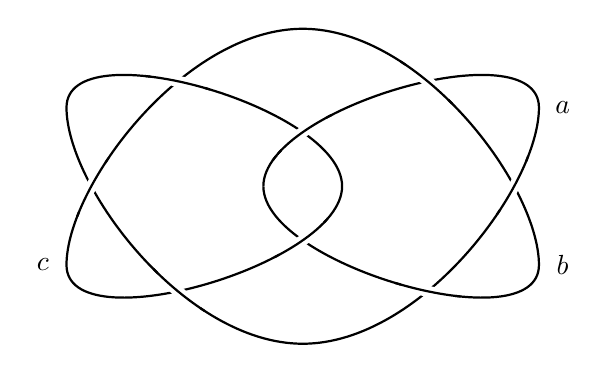
\begin{tikzpicture}
\begin{knot}[consider self intersections = true, clip width = 5, ignore endpoint intersections=false,
%draft mode = crossings,
flip crossing/.list={3, 5, 7}]
\strand[thick] (-0.5, 0) .. controls +(0, 1) and +(0, 1) .. (3, 1) .. controls +(0, -1) and +(1.5, 0) .. (0, -2) .. controls +(-1.5, 0) and +(0, -1) .. (-3, 1) .. controls +(0, 1) and +(0, 1) .. (0.5, 0) .. controls +(0, -1) and +(0, -1) .. (-3, -1) .. controls +(0, 1) and +(-1.5, 0) .. (0, 2) .. controls +(1.5, 0) and +(0, 1) .. (3, -1) .. controls +(0, -1) and +(0, -1) .. (-0.5, 0);
\end{knot}

\node at (3.3, 1) {$a$};
\node at (3.3, -1) {$b$};
\node at (-3.3, -1) {$c$};
\end{tikzpicture}
\end{document}


